\documentclass[10pt]{article}

\usepackage{amsthm}
\usepackage{amsmath}
\usepackage{amssymb}
\usepackage{mathtools}
\usepackage{graphicx}
\usepackage[colorinlistoftodos]{todonotes}
\usepackage{url}
\usepackage{xcolor}
\usepackage[font=small,labelfont=bf]{caption}

\usepackage{pgfplots}

\usepackage[left = 1cm, top = 1cm, bottom = 2cm, right = 1cm, nohead, nofoot]{geometry}

\pgfplotsset{width=20cm, compat=1.9}

\newcommand{\C}{\mathbb{C}}  % Complex
\newcommand{\R}{\mathbb{R}}  % Real
\newcommand{\Z}{\mathbb{Z}}  % Integers
\newcommand{\N}{\mathbb{N}}  % Naturals

\newcommand{\A}{\mathbb{A}}
\newcommand{\K}{\mathbb{K}}

\title{$\A$dvanced $\C$alculus}
\author{$\C$ason $\K$onzer}
\date{December 6, 2021}



\begin{document}
\maketitle

\newpage


%%%%%%%%%%%%%%%%%%%%%%%%%%%%%%%%%%%%%%%%%%%%%%%%%%%%%%%%%%%%%%%%%%%%%%%%%%%%%%%%%%%%%%%%%%%%%%%%
%%%%%%%%%%%%%%%%%%%%%%%%%%%%%%%%%%        Problem #1       %%%%%%%%%%%%%%%%%%%%%%%%%%%%%%%%%%%%%
\section{\underline{}}
\label{sec: Problem 1}

\noindent
The velocity field of a fluid with density $ \rho = 400\ \tfrac{kg}{m^3} $ 
is given by $ \textbf{F}(x,y,z) = \left<1-x,-y,-z-1\right> $ $ \tfrac{m}{s} $. 
Let $ T $ be the polyhedral region with vertices 
$ (0,0,0) $, $ (1,0,0) $, $ (0,1,0) $, and $ (0,0,1) $.  $ S $ is the boundary of $ T $. \\ 
Compute $ \displaystyle \iint \limits_{S} \rho \textbf{F} \cdot \textbf{n}\ dA $ 
by both using the divergence theorem and directly by considering the flux on each face. \\
\vspace{2.5mm}

\hrule 

\vspace{7.5mm}

\noindent
\textbf{First} we will first solve via the divergence theorem. \\

\begin{itemize}
    \item We know by the divergence theorem that 
    $ \displaystyle \rho \iint \limits_{S} \textbf{F} \cdot \textbf{n} \, dA = \rho \iiint \limits_{T} \nabla \cdot \textbf{F} \, dV $ \\
    \item We will first solve for $ \nabla \cdot \textbf{F} $. \\
    \subitem $ \displaystyle \nabla \cdot \textbf{F} = \left<\frac{\partial}{\partial x},\frac{\partial}{\partial y},\frac{\partial}{\partial z}\right> \cdot \left<1-x,-y,-z-1\right> \tfrac{m}{s}= [(1-x)_{x} + (-y)_{y} + (-1-z)_{z}] \tfrac{m}{s} = [-1 -1 -1] \tfrac{m}{s} $ \\
    \subitem $ \displaystyle \nabla \cdot \textbf{F} = -3 \tfrac{m}{s} $ \\
    \item The volume the region $ T $ is $ \displaystyle V = \dfrac{1}{6}m^3 $. \\
    \item We can now put everything together \dots \\
    \subitem $ \displaystyle \rho \cdot \nabla \cdot \textbf{F} \cdot V = 400\ \tfrac{kg}{m^3} \cdot - 3s^{-1} \cdot \dfrac{1}{6}m^3 = -200\tfrac{kg}{s}  $ \\
    \subitem The region is a sink with $ 200kg $ flowing in per second.
\end{itemize}

\noindent
\textbf{Second} we will first solve by considering the flux through each face of $ T $. \\

\begin{itemize}
    \item Consider the face with verticies $ (0,0,0), (1,0,0), (0,1,0) $. \\
    \subitem The unit normal vector at this point is strictly in the $ z $ direction. \\
    \subitem $ \displaystyle \textbf{n} = \left< 0,0,-1 \right> $ \\
    \subitem $ \displaystyle \textbf{F} \cdot \textbf{n} = \left<1-x,-y,-z-1\right> \cdot \left< 0,0,-1 \right> = z + 1 $ \\
    \subitem Across this face $ z $ is a constant of 0 $ \therefore \textbf{F} \cdot \textbf{n} = 1 $ \\
    \subitem This face is a triangle with area $ \displaystyle \frac{1}{2}m^2 $ \\
    \subitem The flux through this face is $ \displaystyle \rho \iint \limits_{S} \textbf{F} \cdot \textbf{n} \, dA = 400\tfrac{kg}{s} \cdot 1\tfrac{m}{s} \cdot \frac{1}{2}m^2 = 200\tfrac{kg}{s} $ \\
    \item Consider the face with verticies $ (0,0,0), (1,0,0), (0,0,1) $. \\
    \subitem The unit normal vector at this point is strictly in the $ z $ direction. \\
    \subitem $ \displaystyle \textbf{n} = \left< 0,-1,0 \right> $ \\
    \subitem $ \displaystyle \textbf{F} \cdot \textbf{n} = \left<1-x,-y,-z-1\right> \cdot \left< 0,-1,0 \right> = y $ \\
    \subitem Across this face $ y $ is a constant of 0 $ \therefore \textbf{F} \cdot \textbf{n} = 0 $ \\
    \subitem This face is a triangle with area $ \displaystyle \frac{1}{2}m^2 $ \\
    \subitem The flux through this face is $ \displaystyle \rho \iint \limits_{S} \textbf{F} \cdot \textbf{n} \, dA = 400\tfrac{kg}{s} \cdot 0\tfrac{m}{s} \cdot \frac{1}{2}m^2 = 0\tfrac{kg}{s} $ \\
    \item Consider the face with verticies $ (0,0,0), (0,1,0), (0,0,1) $. \\
    \subitem The unit normal vector at this point is strictly in the $ z $ direction. \\
    \subitem $ \displaystyle \textbf{n} = \left< -1,0,0 \right> $ \\
    \subitem $ \displaystyle \textbf{F} \cdot \textbf{n} = \left<1-x,-y,-z-1\right> \cdot \left< 0,0,-1 \right> = x - 1 $ \\
    \subitem Across this face $ x $ is a constant of 0 $ \therefore \textbf{F} \cdot \textbf{n} = -1 $ \\
    \subitem This face is a triangle with area $ \displaystyle \frac{1}{2}m^2 $ \\
    \subitem The flux through this face is $ \displaystyle \rho \iint \limits_{S} \textbf{F} \cdot \textbf{n} \, dA = 400\tfrac{kg}{s} \cdot -1\tfrac{m}{s} \cdot \frac{1}{2}m^2 = -200\tfrac{kg}{s} $ \\
    \item Consider the face with verticies $ (1,0,0), (0,1,0), (0,0,1) $. \\
    \subitem The unit normal vector at this point is equal in the $ x,y, $ and $ z $ direction. \\
    \subitem $ \displaystyle \textbf{n} = \left< \frac{1}{\sqrt{3}},\frac{1}{\sqrt{3}},\frac{1}{\sqrt{3}} \right> $ \\
    \subitem $ \displaystyle \textbf{F} \cdot \textbf{n} = \left<1-x,-y,-z-1\right> \cdot \left< \frac{1}{\sqrt{3}},\frac{1}{\sqrt{3}},\frac{1}{\sqrt{3}} \right> =\frac{1}{\sqrt{3}} \Bigl[ 1-x+-y+-z-1 \Bigr] =\frac{1}{\sqrt{3}} \Bigl[ -x+-y+-z \Bigr] $ \\
    \subitem Across this face $ x + y + z $ is a constant of 1 $ \therefore \textbf{F} \cdot \textbf{n} = - \frac{1}{\sqrt{3}}\tfrac{m}{s} $ \\
    \subitem This face is a triangle with area $ \displaystyle \frac{\sqrt{3}}{2}m^2 $ \\
    \subitem The flux through this face is $ \displaystyle \rho \iint \limits_{S} \textbf{F} \cdot \textbf{n} \, dA = 400\tfrac{kg}{m^3} \cdot -\frac{1}{\sqrt{3}}\tfrac{m}{s} \cdot \frac{\sqrt{3}}{2}m^2 = -200\tfrac{kg}{s} $ \\
    \item Last we can find the flux through this surface by summing the flux through each face. \\
    \subitem flux $ \displaystyle = \Bigl[200 + 0 -200 -200\Bigr]\tfrac{kg}{s} = -200\tfrac{kg}{s} $ \\
    \subitem As we oriented the normals directed out of the surface, the negative sign in the flux indicates flow into the surface. \\
    \subitem Again we find that the region is a sink with $ 200kg $ flowing in per second. \\
\end{itemize}

\newpage


%%%%%%%%%%%%%%%%%%%%%%%%%%%%%%%%%%%%%%%%%%%%%%%%%%%%%%%%%%%%%%%%%%%%%%%%%%%%%%%%%%%%%%%%%%%%%%%%
%%%%%%%%%%%%%%%%%%%%%%%%%%%%%%%%%%        Problem #2       %%%%%%%%%%%%%%%%%%%%%%%%%%%%%%%%%%%%%
\section{\underline{}}
\label{sec: Problem 2}

\noindent
Let $ f(x) = -x $ for $ 0 < x < 1 $.  
Find the Fourier series for an \textbf{odd} periodic extension of $ f $, 
listing the first 4 non-zero terms. \\
Then, find the general solution to the ODE $ y'' + y = f(x) $. \\
\vspace{2.5mm}

\hrule 

\vspace{7.5mm}

\noindent
\textbf{First} we will solve for the Fourier series. \\

\begin{itemize}
    \item We know the form of a Fourier series is $ \displaystyle f(x) = a_0 + \sum_{n = 1}^{\infty} a_n \cos(n\pi x/L) + b_n \sin (n\pi x/L) $. \\
    \subitem Here $ L = 1 $ and the function is treated as odd, we now have  $ \displaystyle f(x) = \sum_{n = 1}^{\infty} b_n \sin (n\pi x) $. \\
    \item We also know $ \displaystyle b_n = \frac{2}{L} \int_{0}^{L} f(x) \sin(\frac{n\pi x}{L}) \,dx $. \\
    \subitem Here $ \displaystyle b_n = 2 \int_{0}^{1} -x \sin{(n\pi x)} \,dx $. \\
    \item We can solve the itergral to simplify $ b_n $. \\
    \subitem $ \displaystyle b_n = \frac{\pi  n \cos (\pi  n)-\sin (\pi  n)}{\pi ^2 n^2} $ \\
    \subitem Furthermore; $ \displaystyle \sin (\pi  n) $ is 0 for all integer multiples of $ n $. Thus \dots \\
    \subitem $ \displaystyle b_n = \frac{\cos(\pi n)}{\pi n} $. \\
    \item The Fourier series of $ f $ is then $ \displaystyle f(x) = \sum_{n = 1}^{\infty} \frac{\cos(\pi n)}{\pi n} \sin (n\pi x) $. \\
    \subitem The first 4 terms are $ \displaystyle -\frac{\sin (\pi  x)}{\pi },\frac{\sin (2 \pi  x)}{2 \pi },-\frac{\sin (3 \pi  x)}{3 \pi },\frac{\sin (4 \pi  x)}{4 \pi } $. \\
\end{itemize}

\begin{center}
    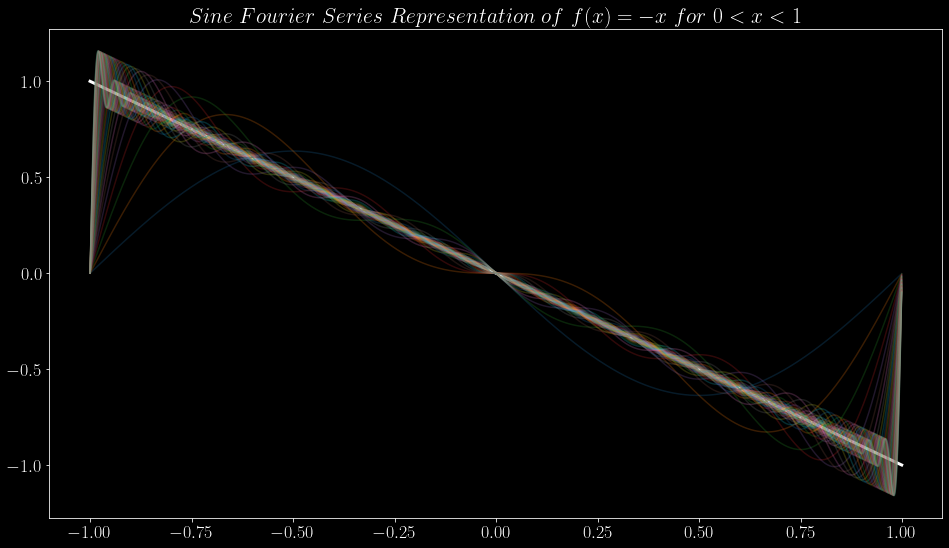
\includegraphics[width=0.72\textwidth]{img/2_1.png} \\
\end{center}

\newpage

\noindent
\textbf{Second} we will solve the ODE. \\

\begin{itemize}
    \item To solve the ODE, we must first solve for a homogeneous solution ; $ \displaystyle y_h \ | \ y'' + y = 0 $. \\
    \subitem $ \displaystyle h^2 + 1 = 0 \ ; \ h^2 = -1 \ ; \ h = \pm i $. \\
    \subitem $ \displaystyle y_h = c_1 cos{(x)} + c_2 sin{(x)} $. \\
    \item Second, we must solve for a particular solution ; $ y_p \ | \ y'' + y = f(x) $. \\
    \subitem $ \displaystyle y = B\sin{(n\pi x)} \ ; \ y' = Bn\pi\cos{(n\pi x)} \ ; \ y'' = -Bn^2\pi^2\sin{(n\pi x)} $. \\
    \item We can now substitute into the origional equation. \\
    \subitem $ \displaystyle -Bn^2\pi^2\sin{(n\pi x)} + B\sin{(n\pi x)} = \frac{\cos(\pi n)}{\pi n} \sin{(n\pi x)} $. \\
    \subitem $ \displaystyle B(1 - n^2\pi^2) = \frac{\cos(\pi n)}{\pi n} \ ; \ B = \frac{\cos(\pi n)}{\pi n(1 - n^2\pi^2)} ; $ We can notice here that $ \cos{(n\pi)} = (-1)^n $. \\
    \subitem $ \displaystyle B = \frac{(-1)^n}{n\pi - n^3\pi^3} $. \\
    \item From here we can solve for the particular solution $ \displaystyle y_p = \sum_{n = 1}^{\infty} B \sin (n\pi x) $. \\
    \subitem $ \displaystyle y_p = \sum_{n = 1}^{\infty} \frac{(-1)^n\sin (n\pi x)}{n\pi - n^3\pi^3} $. \\
    \item Combining the homogeneous and particular solution, we have the general solution $ \displaystyle y = y_h + y_p $. \\
    \subitem  $ \displaystyle y = c_1 cos{(x)} + c_2 sin{(x)} + \sum_{n = 1}^{\infty} \frac{(-1)^n\sin (n\pi x)}{n\pi - n^3\pi^3} $. \\
\end{itemize}

\begin{center}
    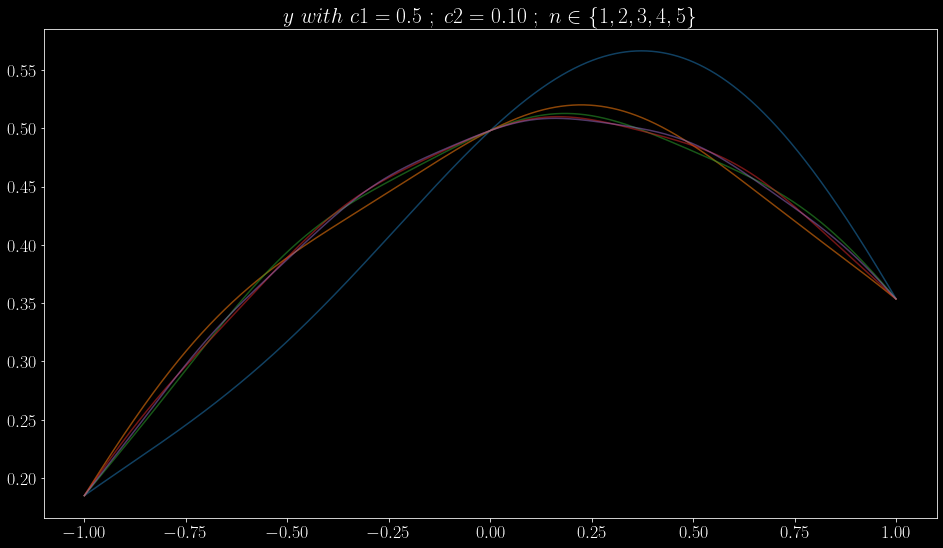
\includegraphics[width=0.72\textwidth]{img/2_2.png} \\
\end{center}

\newpage


%%%%%%%%%%%%%%%%%%%%%%%%%%%%%%%%%%%%%%%%%%%%%%%%%%%%%%%%%%%%%%%%%%%%%%%%%%%%%%%%%%%%%%%%%%%%%%%%
%%%%%%%%%%%%%%%%%%%%%%%%%%%%%%%%%%        Problem #3       %%%%%%%%%%%%%%%%%%%%%%%%%%%%%%%%%%%%%
\section{\underline{}}
\label{sec: Problem 3}

\noindent
Use the Fourier sine transform to derive the solution formula for the heat equation 
$ u_{t} = c^2u_{xx} $ on the half-infinite bar ($ 0 \le x < \infty $) 
with Dirichlet boundary condition $ u(0,t) = a $, for some constant $ a $, 
and initial condition $ u(x,0) = f(x) $. \\
\vspace{2.5mm}

\hrule 

\vspace{7.5mm}

\noindent
\textbf{First} transfrom the PDE to an ODE by the Fourier sine transform. \\

\begin{itemize}
    \item $ \mathcal{F}_{s}\{ u_{t} \} = \mathcal{F}_{s}\{ c^2 u_{tt} \} $. \\
    \subitem $ \displaystyle \dot{\hat{u}}_{s} = c^2\Bigl[-w^{2}\hat{u}_{s} + \sqrt{\frac{2}{\pi}}wu(0,t) \Bigr] $ \\
    \subitem $ \displaystyle \dot{\hat{u}}_{s} = -w^2c^2\hat{u}_{s} + awc^2\sqrt{\frac{2}{\pi}} $ \\
    \subitem $ \displaystyle \dot{\hat{u}}_{s} + w^2c^2\hat{u}_{s} = awc^2\sqrt{\frac{2}{\pi}} $ \\
    \item Solve for the homogeneous solution $ (\hat{u}_{s})_{h} \ | \ \dot{\hat{u}} + w^2c^2\hat{u}_{s} = 0 $ \\
    \subitem $ \displaystyle \lambda = -w^2c^2 $ \\
    \subitem $ \displaystyle (\hat{u}_{s})_{h} = \kappa(w)e^{\lambda t} $ \\
    \subitem $ \displaystyle (\hat{u}_{s})_{h}(w,0) = \mathcal{F}_{s}\{ u(x,0) \} = \mathcal{F}_{s}\{ f(x) \} = \hat{f}_{s}(w) $ \\
    \subitem $ \displaystyle (\hat{u}_{s})_{h} = \hat{f}_{s}(w)e^{-w^2c^2t} $ \\
    \item Solve for the particular solution $ (\hat{u}_{s})_{p} \ | \ \dot{\hat{u}} + w^2c^2\hat{u}_{s} = awc^2\sqrt{\frac{2}{\pi}} $ \\
    \subitem $ \displaystyle (\hat{u}_{s})_{p} = \kappa(w) $ \\
    \subitem $ \displaystyle (\dot{\hat{u}}_{s})_{p} = 0 $ \\
    \subitem $ \displaystyle 0 + w^2c^2\kappa(w) = awc^2\sqrt{\frac{2}{\pi}} $ \\
    \subitem $ \displaystyle \kappa(w) = \frac{awc^2\sqrt{\frac{2}{\pi}}}{w^2c^2} = \frac{a}{w}\sqrt{\frac{2}{\pi}} $ \\
    \subitem $ \displaystyle (\hat{u}_{s})_{p} = \frac{a}{w}\sqrt{\frac{2}{\pi}} $ \\
    \item Combining the homogeneous and particular solution, we have the general solution $ \displaystyle \hat{u}_{s} = (\hat{u}_{s})_{h} + (\hat{u}_{s})_{p} $. \\
    \subitem $ \displaystyle \hat{u}_{s} = \hat{f}_{s}e^{-w^2c^2t} + \frac{a}{w}\sqrt{\frac{2}{\pi}} $ \\

\newpage

    \item We know the form of $ \displaystyle \hat{f}_{s}(w) = \sqrt{\frac{2}{\pi}} \int \limits_{0}^{\infty} f(p)\sin{(wp)} \, dp $ \\
    \subitem $ \displaystyle \hat{u}_{s}(w,t) = \sqrt{\frac{2}{\pi}} \Bigl[ \int \limits_{0}^{\infty} f(p)\sin{(wp)} \, dp \Bigr]e^{-w^2c^2t} + \frac{a}{w}\sqrt{\frac{2}{\pi}} $ \\
    \subitem $ \displaystyle \hat{u}_{s}(w,t) = \sqrt{\frac{2}{\pi}} \Bigl[ e^{-w^2c^2t} \int \limits_{0}^{\infty} f(p)\sin{(wp)} \, dp + \frac{a}{w} \Bigr] $ \\
    \item We can now transfer back into $ \displaystyle u(x,t) $ as $ \displaystyle u(x,t) = \mathcal{F}_{s}^{-1}\{ \hat{u_{s}}(w,t) \} \ ; \ f(x) = \mathcal{F}_{s}^{-1}\{f(w)\} = \sqrt{\frac{2}{\pi}} \int \limits_{0}^{\infty} f(w)\sin{(wx)} \, dw $ \\
    \subitem $ \displaystyle u(x,t) = \sqrt{\frac{2}{\pi}} \int \limits_{0}^{\infty} \Biggl[ \sqrt{\frac{2}{\pi}} \Bigl[ e^{-w^2c^2t} \int \limits_{0}^{\infty} f(p)\sin{(wp)} \, dp + \frac{a}{w} \Bigr] \Biggr]\sin{(wx)} \, dw $ \\
    \subitem $ \displaystyle u(x,t) = \frac{2}{\pi} \int \limits_{0}^{\infty} \Biggl[ \Bigl[ e^{-w^2c^2t} \int \limits_{0}^{\infty} f(p)\sin{(wp)} \, dp + \frac{a}{w} \Bigr] \Biggr]\sin{(wx)} \, dw $ \\
\end{itemize}

\newpage


%%%%%%%%%%%%%%%%%%%%%%%%%%%%%%%%%%%%%%%%%%%%%%%%%%%%%%%%%%%%%%%%%%%%%%%%%%%%%%%%%%%%%%%%%%%%%%%%
%%%%%%%%%%%%%%%%%%%%%%%%%%%%%%%%%%        Problem #4       %%%%%%%%%%%%%%%%%%%%%%%%%%%%%%%%%%%%%
\section{\underline{}}
\label{sec: Problem 4}

\noindent
Once the temperature in an object reaches a steady state, 
the heat equation becomes the Laplace equation.  
Use separation of variables to derive the steady-state solution to the heat equation on the rectangle 
$ R = [0,1] \times [0,1] $ with the following Dirichlet boundary conditions: 
$ u = 0 $ on the left and right sides; 
$ u = f(x) $ on the bottom; 
$ u = g(x) $ on the top. 
That is, solve $ u_{xx} + u_{yy} = 0 $ subject to 
$ u(0,y) = u(1,y) = 0 $, $ u(x,0) = f(x) $, and $ u(x,1) = g(x) $. 
You may assume the separation constant is negative: $ F'' / F = -k $, for $ k > 0 $. 
Finally, plot $ u(x,y) $ when $ f(x) = \sin{(\pi x)} $ and $ g(x) = \sin{(3\pi x)} $. \\
\vspace{2.5mm}

\hrule 

\vspace{7.5mm}

\noindent
\textbf{First} we will use seperation of variable to obtain 2 ODEs. \\

\begin{itemize}
    \item Assume $ \displaystyle u(x,y) = F(x)G(y) $ solve for the partial derivates \dots \\
    \subitem $ \displaystyle u_{x} = F'G $ \\
    \subitem $ \displaystyle u_{xx} = F''G $ \\   
    \subitem $ \displaystyle u_{y} = FG' $ \\
    \subitem $ \displaystyle u_{yy} = FG'' $ \\
    \item Substitute into the know equation $ \displaystyle u_{xx} + u_{yy} = 0 $. \\
    \subitem $ \displaystyle F''G + FG'' = 0 $ \\
    \subitem $ \displaystyle F''G = - FG''$ \\ 
    \subitem $ \displaystyle \frac{F''}{F} =  - \frac{G''}{G} = -k $ \\
    \subitem $ \displaystyle F'' = -kF \ ; \ G'' = kG $ \\
    \item Solve the ODEs\dots \\
    \subitem $ \displaystyle \lambda_{f}^2 = -k \ ; \ \lambda_{g}^2 = k $ \\
    \subitem $ \displaystyle \lambda_{f} = \pm i \sqrt{k} \ ; \ \lambda_{g} = \pm \sqrt{k} $ \\
    \subitem $ \displaystyle F(x) = A_{f}\cos{(x\sqrt{k})} + B_{f}\sin{(x\sqrt{k})} \ ; \ G(y) = A_{g}e^{y\sqrt{k}} + B_{g}e^{-y\sqrt{k}} $ \\
    \item Inspect the initial conditions \dots \\
    \subitem $ \displaystyle u(0,y) = 0 \Rightarrow F(0)G(y) = 0 \Rightarrow F(0) = 0 $ \\
    \subitem $ \displaystyle u(1,y) = 0 \Rightarrow F(1)G(y) = 0 \Rightarrow F(1) = 0 $ \\
    \subitem $ \displaystyle u(x,0) = f(x) \Rightarrow F(x)G(0) = f(x) $ \\
    \subitem $ \displaystyle u(x,1) = g(x) \Rightarrow F(x)G(1) = g(x) $ \\
    \item Use the initial conditions to simplify $ F $ and $ G $. \\
    \subitem $ \displaystyle F(0) = A_{f}\cos{(0)} + B_{f}\sin{(0)} = A_{f} = 0 \Rightarrow F(x) = B_{f}\sin{(x\sqrt{k})} $ \\
    \subitem $ \displaystyle F(1) = B_{f}\sin{(\sqrt{k})} = 0 \Rightarrow \sqrt{k}_n = n\pi \Rightarrow F_n(x) = B_{f_n}\sin{(n\pi x)} $ \\
    \subitem $ \displaystyle G(0) = A_{g} + B_{g} = f(x) $ \\
    \subitem $ \displaystyle G(1) = A_{g}e^{n\pi } + B_{g}e^{-n\pi } = g(x) $ \\
    \subitem $ \displaystyle G_n(y) = A_{g_n}e^{yn\pi} + B_{g_n}e^{-yn\pi} $ \\
    \item Find the form of $ u $. \\
    \subitem $ \displaystyle u_n(x,y) = F_n(x)G_n(y) = B_{f_n}\sin{(n\pi x)}\Bigl[A_{g_n}e^{yn\pi} + B_{g_n}e^{-yn\pi}\Bigr] $ \\
    \subitem $ \displaystyle u_n(x,y) = \sin{(n\pi x)}\Bigl[A_{n}e^{yn\pi } + B_{n}e^{-yn\pi }\Bigr] $ \\
    \subitem $ \displaystyle u(x,y) = \sum \limits_{n=1}^{\infty} \sin{(n\pi x)}\Bigl[A_{n}e^{yn\pi } + B_{n}e^{-yn\pi }\Bigr] $ \\
    \item Use the initial conditions to find the constants $ A_n $ and $ B_n $. \\
    \subitem $ \displaystyle u(x,0) = f(x) = \sum \limits_{n=1}^{\infty} \sin{(n\pi x)}\Bigl[A_{n} + B_{n}\Bigr] $ \\
    \subitem $ \displaystyle A_{n} + B_{n} = 2 \int \limits_{0}^{1} f(x) \sin{(n\pi x)} \,dx $ \\
    \subitem $ \displaystyle A_{n} = 2 \int \limits_{0}^{1} f(x) \sin{(n\pi x)} \,dx - B_{n} $ \\
    \subitem $ \displaystyle u(x,1) = g(x) = \sum \limits_{n=1}^{\infty} \sin{(n\pi x)}\Bigl[A_{n}e^{n\pi} + B_{n}e^{-n\pi}\Bigr] $ \\ 
    \subitem $ \displaystyle A_{n}e^{n\pi} + B_{n}e^{-n\pi} = 2 \int \limits_{0}^{1} g(x) \sin{(n\pi x)} \,dx $ \\
    \subitem $ \displaystyle 2 \int \limits_{0}^{1} f(x) \sin{(n\pi x)}e^{n\pi} \,dx - B_{n}e^{n\pi} + B_{n}e^{-n\pi} = 2 \int \limits_{0}^{1} g(x) \sin{(n\pi x)} \,dx $ \\
    \subitem $ \displaystyle  B_{n}\Bigl[e^{-n\pi} - e^{n\pi}\Bigr] = 2 \int \limits_{0}^{1} g(x) \sin{(n\pi x)} \,dx - 2 \int \limits_{0}^{1} f(x) \sin{(n\pi x)}e^{n\pi} \,dx $ \\
    \subitem $ \displaystyle  B_{n} = \frac{2 \int \limits_{0}^{1} [g(x) - f(x)e^{n\pi}]\sin{(n\pi x)} \,dx }{e^{-n\pi} - e^{n\pi}} $ \\
    \subitem $ \displaystyle  A_{n} = 2 \int \limits_{0}^{1} f(x)\sin{(n\pi x)} \,dx - \frac{2 \int \limits_{0}^{1} [g(x) - f(x)e^{n\pi}]\sin{(n\pi x)} \,dx }{e^{-n\pi} - e^{n\pi}} $
    \subitem $ \displaystyle  A_{n} = \frac{2 \int \limits_{0}^{1} [f(x)[e^{-n\pi} - e^{n\pi}] - g(x) - f(x)e^{n\pi}]\sin{(n\pi x)} \,dx }{e^{-n\pi} - e^{n\pi}} $ \\
    \subitem $ \displaystyle  A_{n} = \frac{2 \int \limits_{0}^{1} [f(x)e^{-n\pi} - 2f(x)e^{n\pi} - g(x)]\sin{(n\pi x)} \,dx }{e^{-n\pi} - e^{n\pi}} $ \\
    \item Substitue $ A_n $ and $ B_n $ into $ u(x,t) $. \\
    \subitem $ \displaystyle u(x,y) = \sum \limits_{n=1}^{\infty} \sin{(n\pi x)}\Bigl[\frac{2e^{yn\pi } \int \limits_{0}^{1} [f(x)e^{-n\pi} - 2f(x)e^{n\pi} - g(x)]\sin{(n\pi x)} \,dx }{e^{-n\pi} - e^{n\pi}} + \frac{2e^{-yn\pi } \int \limits_{0}^{1} [g(x) - f(x)e^{n\pi}]\sin{(n\pi x)} \,dx }{e^{-n\pi} - e^{n\pi}}\Bigr] $ \\
    \subitem $ \displaystyle u(x,y) = 2\sum \limits_{n=1}^{\infty} \sin{(n\pi x)}\Bigl[\frac{e^{yn\pi } \int \limits_{0}^{1} [f(x)e^{-n\pi} - 2f(x)e^{n\pi} - g(x)]\sin{(n\pi x)} \,dx + e^{-yn\pi } \int \limits_{0}^{1} [g(x) - f(x)e^{n\pi}]\sin{(n\pi x)} \,dx }{e^{-n\pi} - e^{n\pi}}\Bigr] $ \\
    \item Solving for $ u(x,y) $ when $ f(x) = \sin{(\pi x)} $ and $ g(x) = \sin{(3\pi x)} \dots$ \\
    \subitem $ \displaystyle  B_{n} = \frac{2 \int \limits_{0}^{1} [\sin{(3\pi x)} - \sin{(\pi x)}e^{n\pi}]\sin{(n\pi x)} \,dx }{e^{-n\pi} - e^{n\pi}} = \frac{2 \left(\frac{3}{9 \pi -\pi  n^2}+\frac{e^{n\pi}}{\pi  \left(n^2-1\right)}\right) \sin (\pi  n)}{e^{-n\pi}-e^{n\pi}} $ \\
    \subitem $ \displaystyle A_{n} = 2 \int \limits_{0}^{1} \sin{(\pi x)} \sin{(n\pi x)} \,dx - B_{n} = \frac{2 \sin (\pi  n)}{\pi -\pi  n^2} - B_n = 2\sin{(n\pi)} \Biggl[ \frac{1}{\pi -\pi  n^2} - \frac{ \left(\frac{3}{9 \pi -\pi  n^2}+\frac{e^{n\pi}}{\pi  \left(n^2-1\right)}\right)}{e^{-n\pi}-e^{n\pi}} \Biggr] $ \\
    \subitem $ \displaystyle A_{n} = 2\sin{(n\pi)} \Biggl[ \frac{(\pi -\pi  n^2) - \left(\frac{3}{9 \pi -\pi  n^2}+\frac{e^{\pi  n}}{\pi  \left(n^2-1\right)}\right)}{\pi(1 - n^2)(e^{-n\pi}-e^{n\pi})} \Biggr] $ \\
    \subitem $ \displaystyle u(x,y) = \sum \limits_{n=1}^{\infty} \sin{(n\pi x)}\Bigl[A_{n}e^{yn\pi } + B_{n}e^{-yn\pi }\Bigr] $ \\
\end{itemize}

\begin{center}
    \begin{minipage}{0.49\linewidth}
        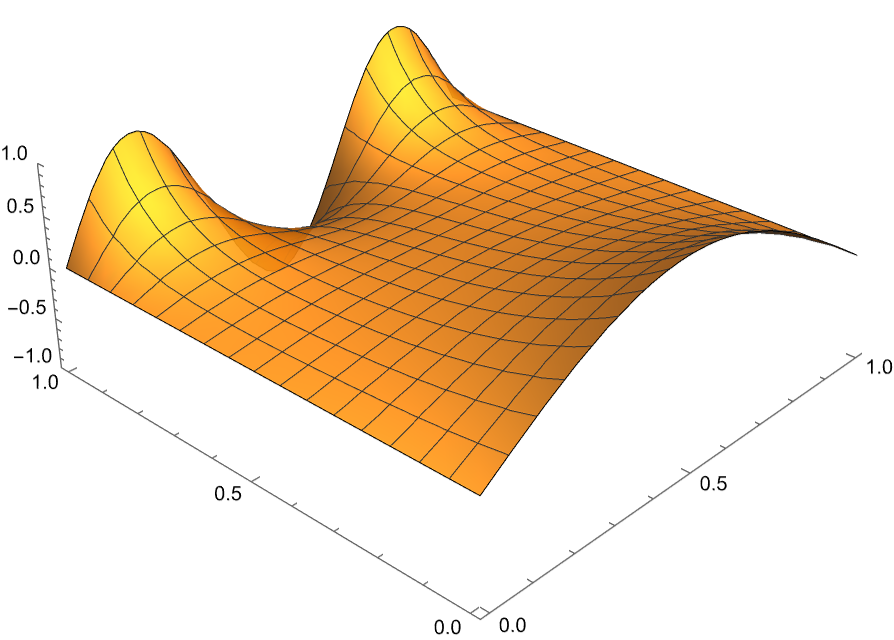
\includegraphics[width=\textwidth]{img/4_2.png}
    \end{minipage}
    \hfill
    \begin{minipage}{0.49\linewidth}
        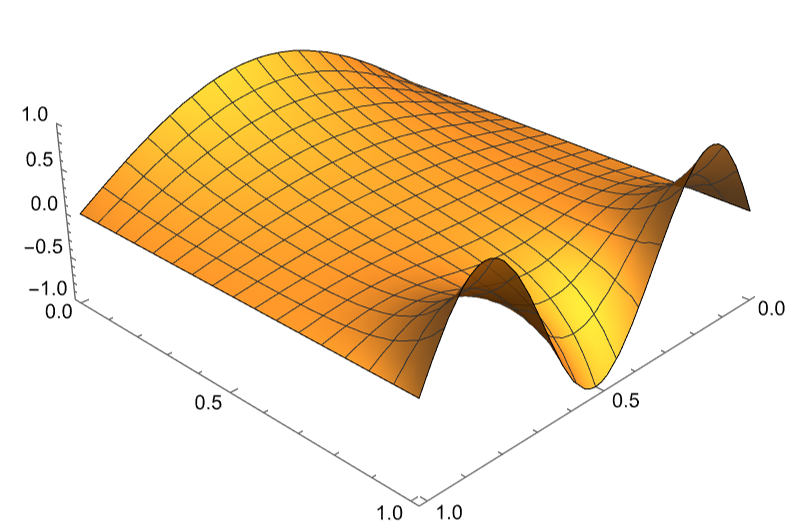
\includegraphics[width=.96\textwidth]{img/4_1.png}
    \end{minipage}
\end{center}

\newpage


%%%%%%%%%%%%%%%%%%%%%%%%%%%%%%%%%%%%%%%%%%%%%%%%%%%%%%%%%%%%%%%%%%%%%%%%%%%%%%%%%%%%%%%%%%%%%%%%
%%%%%%%%%%%%%%%%%%%%%%%%%%%%%%%%%%        Problem #5       %%%%%%%%%%%%%%%%%%%%%%%%%%%%%%%%%%%%%
\section{\underline{}}
\label{sec: Problem 5}

\noindent
Let $ \displaystyle u(x,t) $ be the solution to $ \displaystyle u_{tt} = 16u_{xx} $ 
for $ \displaystyle 0 \leq x \leq 2 $ and $ \displaystyle t \geq 0 $, 
where: $ \displaystyle u(0,t) = 0 $, $ u(2,t) = 0 $, and $ \displaystyle u(x,0) = f(x) = 1 - |x-1| $ 
for $ \displaystyle 0 \le x \le 2 $. Use D'Alembert's solution to find $ \displaystyle u(1,0.1) $ and $ \displaystyle u(1,0.6) $. 
Be careful to consider that D'Alembert's solution uses the odd periodic extension of $ \displaystyle f(x) $. \\
\vspace{2.5mm}

\hrule 

\vspace{7.5mm}

\noindent
\textbf{First} consider the form of the $ f(x) $ extended as an odd function. \\

\begin{center}
    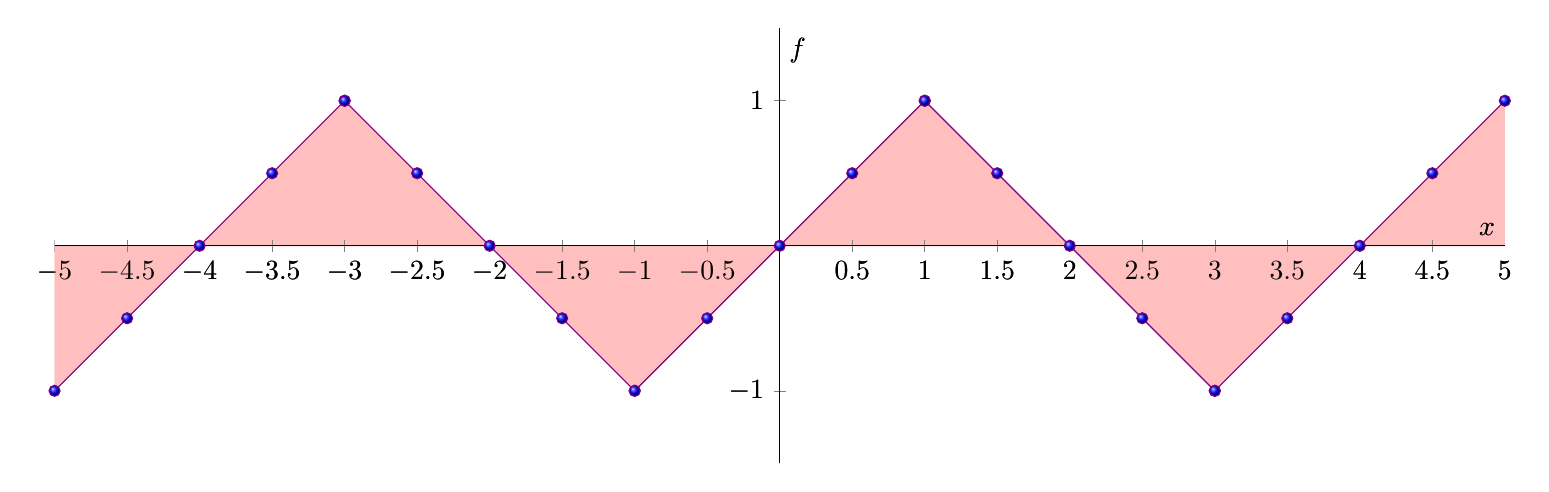
\begin{tikzpicture}
        \begin{axis}[
            xlabel = $ x $, ylabel = $ f $,
            xmin = -5, xmax = 5,
            ymin = -1.5 , ymax = 1.5,
            try min ticks =  2,
            axis equal image = true,
            axis x line=center,
            axis y line=center,
            axis line style = -,
        ]
            \addplot[
                no marks,
                color = pink,
                fill
            ]
                expression[
                    domain = -5 : -3,
                    samples = 3
                ]
                    {x+4}
                \closedcycle
            ;
            \addplot[
                no marks,
                color = pink,
                fill
            ]
                expression[
                    domain = -3 : -1,
                    samples = 3
                ]
                    {-x-2}
                \closedcycle
            ;
            \addplot[
                no marks,
                color = pink,
                fill
            ]
                expression[
                    domain = -1 : 1,
                    samples = 3
                ]
                    {x}
                \closedcycle
            ;
            \addplot[
                no marks,
                color = pink,
                fill
            ]
                expression[
                    domain = 1 : 3,
                    samples = 3
                ]
                    {-x+2}
                \closedcycle
            ;
            \addplot[
                no marks,
                color = pink,
                fill
            ]
                expression[
                    domain = 3 : 5,
                    samples = 3
                ]
                    {x-4}
                \closedcycle
            ;
        \end{axis}
        \begin{axis}[
            xlabel = $ x $, ylabel = $ f $,
            xmin = -5, xmax = 5,
            ymin = -1.5 , ymax = 1.5,
            try min ticks =  2,
            axis equal image = true,
            axis x line=center,
            axis y line=center,
            axis line style = -,
        ]
            \addplot[
                mark = ball,
                color = violet
            ]
                expression[
                    domain = -5 : -3,
                    samples = 5
                ]
                    {x+4}
            ;
            \addplot[
                mark = ball,
                color = violet
            ]
                expression[
                    domain = -3 : -1,
                    samples = 5
                ]
                    {-x-2}
            ;
            \addplot[
                mark = ball,
                color = violet
            ]
                expression[
                    domain = -1 : 1,
                    samples = 5
                ]
                    {x}
            ;
            \addplot[
                mark = ball,
                color = violet
            ]
                expression[
                    domain = 1 : 3,
                    samples = 5
                ]
                    {-x+2}
            ;
            \addplot[
                mark = ball,
                color = violet
            ]
                expression[
                    domain = 3 : 5,
                    samples = 5
                ]
                    {x-4}
            ;
        \end{axis}
    \end{tikzpicture} \\
\end{center}

\noindent
\textbf{Second} we can evaluate given the D'Alembert's solution : $ 2u(x,t) = f(x-ct) + f(x+ct). $ \\

\begin{itemize}
    \item Note that from the equation given, $ \displaystyle c^2 = 16 $, Thus $ \displaystyle c = 4 $. \\
    \item Evaluate $ \displaystyle u(1,0.1) $. \\
    \subitem $ \displaystyle 2u(1,0.1) = f(1-4(0.1)) + f(1+4(0.1)) = f(1-0.4) + f(1+0.4) $ \\
    \subitem $ \displaystyle 2u(1,0.1) = f(0.6) + f(1.4) = 0.6 + 0.6 = 2(0.6) $ \\
    \subitem $ \displaystyle u(1,0.1) = 0.6 $ \\
    \item Evaluate $ \displaystyle u(1,0.6) $. \\
    \subitem $ \displaystyle 2u(1,0.6) = f(1-4(0.6)) + f(1+4(0.6)) = f(1-2.4) + f(1+2.4) $ \\
    \subitem $ \displaystyle 2u(1,0.6) = 0.6 - 0.6 = 0 $ \\
    \subitem $ \displaystyle u(1,0.6) = 0 $ \\
\end{itemize}

\newpage


%%%%%%%%%%%%%%%%%%%%%%%%%%%%%%%%%%%%%%%%%%%%%%%%%%%%%%%%%%%%%%%%%%%%%%%%%%%%%%%%%%%%%%%%%%%%%%%%
%%%%%%%%%%%%%%%%%%%%%%%%%%%%%%%%%%        Problem #6       %%%%%%%%%%%%%%%%%%%%%%%%%%%%%%%%%%%%%
\section{\underline{}}
\label{sec: Problem 6}

\noindent
Find the general solution of $ \displaystyle u_{xx} - 3u_{xy} + 2u_{yy} = 0 $ using the  the method of characteristics: 
let $ \displaystyle v = y + 2x $ and $ \displaystyle w = y + x $; 
define $ \displaystyle U(v,w) $ to be $ \displaystyle U(v,w) = U(y + 2x,y + x) = u(x,y) $; 
derive and solve a PDE for $ \displaystyle U(v,w) $; 
convert back to $ \displaystyle u(x,y) $. 
Use your solution to provide a non-trivial example of a solution. \\
\vspace{2.5mm}

\hrule 

\vspace{7.5mm}

\noindent
\textbf{Solve for u}. \\

\begin{itemize}
    \item We will classify based on the characteristic classifier; $ \displaystyle 4AC - B^2 $. \\
    \subitem $ \displaystyle A = 1 \ ; \ B = -3 \ ; \ C = 2 $ \\
    \subitem $ \displaystyle 4AC - B^2 = 4(1)(2) - (-3)^2 = 8 - 9 = -1 $ \\
    \subitem The PDE is Hyperbolic. $ \Rightarrow $ Target $ U_{vw} = 0 $. \\
    \item Solve for $ \displaystyle x $ and $ \displaystyle y $ in terms of $ \displaystyle u $ and $ \displaystyle v $. \\
    \subitem $ \displaystyle v - w = y + 2x -(y + x) = y + 2x - y - x $ \\
    \subsubitem $ \displaystyle x = v - w $ \\
    \subitem $ \displaystyle y = v - 2x = v - 2(v - w) = v - 2v + 2w $ \\
    \subsubitem $ \displaystyle y = 2w - v $ \\
    \item Solve for the partials of $ \displaystyle x $ and $ \displaystyle y $ with respect to $ \displaystyle v $ and $ \displaystyle w $. \\
    \subitem $ \displaystyle x_{v} = 1 $ \\
    \subitem $ \displaystyle x_{w} = -1 $ \\
    \subitem $ \displaystyle y_{v} = -1 $ \\
    \subitem $ \displaystyle y_{w} = 2 $ \\
    \item Solve for the partials of $ \displaystyle U $. \\
    \subitem $ \displaystyle U_{v} = U_{x}x_{v} + U_{y}y_{v} = U_{x} - U_{y} $ \\
    \subitem $ \displaystyle U_{vv} = (U_{x} - U_{y})_{x}x_{v} + (U_{x} - U_{y})_{y}y_{v} = (U_{x} - U_{y})_{x} - (U_{x} - U_{y})_{y} = U_{xx} - U_{yx} - U_{xy} + U_{yy} = U_{xx} - 2U_{xy} + U_{yy} $ \\
    \subitem $ \displaystyle U_{vw} = (U_{x} - U_{y})_{x}x_{w} + (U_{x} - U_{y})_{y}y_{w} =  2(U_{x} - U_{y})_{y} - (U_{x} - U_{y})_{x} = 2U_{xy} - 2U_{yy} - U_{xx} + U_{yx} = -U_{xx} + 3U_{xy} - 2U_{yy} $ \\
    \subitem $ \displaystyle U_{w} = U_{x}x_{w} + U_{y}y_{w} = 2U_{y} - U_{x} $ \\
    \subitem $ \displaystyle U_{ww} = (2U_{y} - U_{x})_{x}x_{w} + (2U_{y} - U_{x})_{y}y_{w} = 2(2U_{y} - U_{x})_{y} - (2U_{y} - U_{x})_{x} = 4U_{yy} - U_{xy} - 2U_{yx} - U_{xx} = - U_{xx} - 3U_{xy} + 4U_{yy} $ \\
    \item At this point we leverage the form of the PDE. \\
    \subitem $ \displaystyle -U_{vw} = u_{xx} - 3u_{xy} + 2u_{yy} = 0 = U_{vw}$ \\
    \item Integrate to get back to $ U $ \\
    \subitem $ \displaystyle U_{v} = \phi(v) $ \\
    \subitem $ \displaystyle U(v,w) = v\phi(v) + \psi(w) $ \\
    \item Substitue $ \displaystyle v = y + 2x \ ; \ w = y + x $ into $\displaystyle U $ to obtain $ \displaystyle u $. \\
    \subitem $ \displaystyle U(y+2x,y+x) = (y+2x)\phi(y+2x) + \psi(y+x) $ \\
    \subitem $ \displaystyle u(x,y) = y\phi(y+2x) + 2x\phi(y+2x) + \psi(y+x) $ \\
\end{itemize}

\textbf{Find a non-trivial example of u}. \\
\begin{itemize}
    \item $ \displaystyle u(x,y) = y\sin{(y+2x)} + 2x\sin{(y+2x)} - (y+x)^2 $. \\
\end{itemize}

\begin{center}
    \begin{minipage}{0.49\linewidth}
        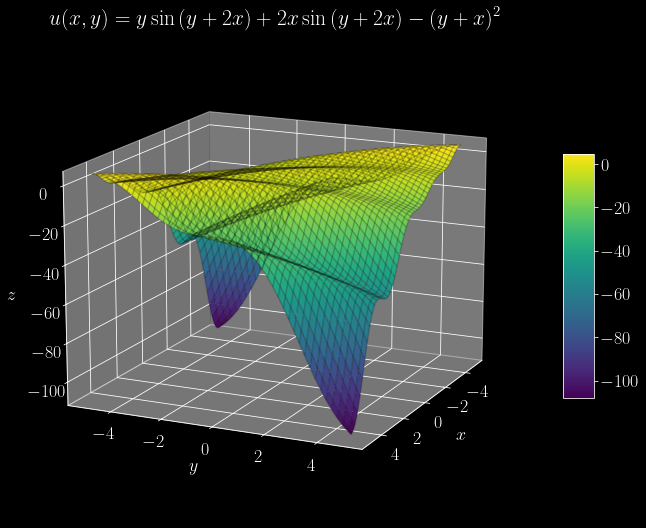
\includegraphics[width=\textwidth]{img/6_1.png}
    \end{minipage}
    \hfill
    \begin{minipage}{0.49\linewidth}
        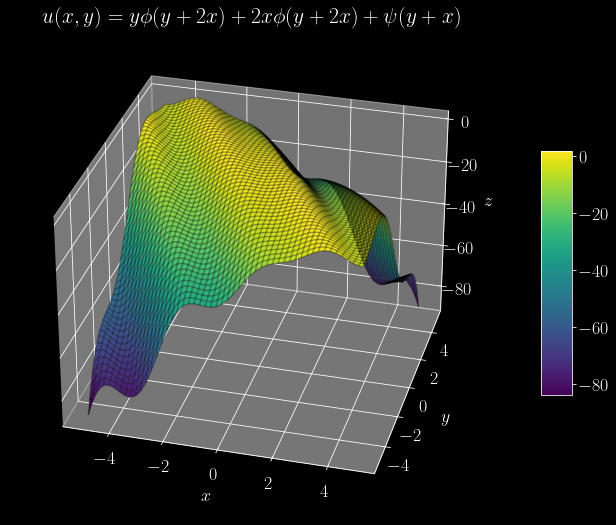
\includegraphics[width=.96\textwidth]{img/6_2.png}
    \end{minipage}
\end{center}

\newpage


\end{document}


%%%%%%%%%%%%%%%%%%%%%%%%%%%%%%%%%%%%%%%%%%%%%%%%%%%%%%%%%%%%%%%%%%%%%%%%%%%%%%%%%%%%%%%%%%%%%%%%
%%%%%%%%%%%%%  Comments - November 13, 2021 Advanced Calculus Written Home Work #7  %%%%%%%%%%%%%